% Canonical starting point for an ML method figure.
% Copy this file into figures/<name>.tex and edit the copy.
%
% Everything below is load-bearing: the palette is colourblind-safe, the arrow
% styles are sized so tips track line width, `bending` is required for curved
% paths, and the parameters block is where all spacing lives. See
% references/method-figure/by-construction.md for why.
%
% Build:  xelatex -interaction=nonstopmode -halt-on-error <name>.tex
% Gate:   scripts/method-figure/qa.sh <name>.tex --venue iclr

\documentclass[tikz,border=10pt]{standalone}

\usepackage{amsmath}
\usepackage{newtxtext,newtxmath}   % match a Times-based paper; drop for sans

% `bending` is NOT optional: without it, arrow tips on any curved or bent path
% render visibly misaligned.
\usetikzlibrary{arrows.meta,bending,calc,fit,positioning,backgrounds}

% ============================================================================
% PALETTE  — the single place colour is defined. Never inline a hex below this.
% Okabe-Ito, colourblind-safe (Wong, Nat. Methods 2011).
%   accent  = the novel contribution, used sparingly
%   primary = main data path
%   second  = auxiliary / context
%   ink     = structure: outlines, text, arrows
% Note: okYellow and okSkyBlue do not reach 3:1 on white — do not use them for
% thin lines or small glyphs without also encoding by shape or line style.
% ============================================================================
\definecolor{okBlue}{HTML}{0072B2}
\definecolor{okOrange}{HTML}{E69F00}
\definecolor{okGreen}{HTML}{009E73}
\definecolor{okPurple}{HTML}{CC79A7}
\definecolor{ink}{HTML}{292C30}
\definecolor{gray}{HTML}{757575}

% ============================================================================
% PARAMETERS — all spacing lives here. Change a value, the figure reflows.
% ============================================================================
\newlength{\boxw}\setlength{\boxw}{2.2cm}
\newlength{\boxh}\setlength{\boxh}{0.7cm}
\newlength{\pad}\setlength{\pad}{0.25cm}      % per-side text padding (min 0.25cm)
\def\colgap{1.5cm}                            % same-row sibling gap (min 1.5cm)
\def\rowgap{1.2cm}                            % cross-row gap (min 1.2cm)
\def\bendr{5pt}                               % the one canonical corner radius

\begin{document}
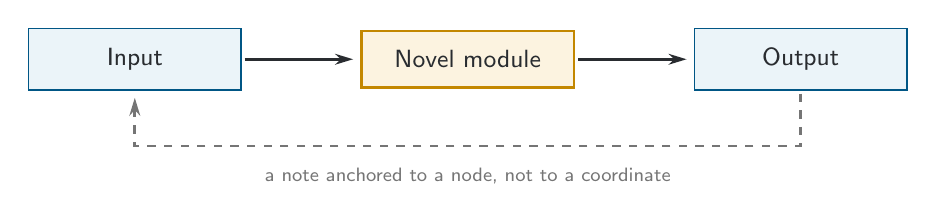
\begin{tikzpicture}[
  font=\sffamily\small,                       % relative size; NEVER absolute pt
  text=ink,
  node distance=\colgap,
%
  % --- arrows -------------------------------------------------------------
  % Tip length is expressed as 5pt + 1.5x line width, so it tracks the stroke.
  % Tune line width, not tip scale. See constraints.md section B.
  flow/.style   ={-{Stealth[length=5pt 1.5,width'=0pt 0.6,sep=0pt 0.5]},
                  line width=1.0pt,shorten >=2pt,shorten <=1pt,draw=ink},
  flow2/.style  ={flow,line width=0.6pt},     % secondary
  emph/.style   ={flow,line width=1.6pt},     % emphasis
  % MANDATORY below 1.5cm: the default tip would leave ~5.5pt of stem.
  short/.style  ={-{Stealth[length=3pt 1.0,width'=0pt 0.5,sep=0pt 0.3]},
                  line width=0.8pt,shorten >=1pt,shorten <=0pt,draw=ink},
  % supervision / privileged / optional: ALWAYS legend-defined (see ml-conventions.md)
  aux/.style    ={flow,dashed,draw=gray},
  % annotation leader: dotted, no arrowhead, association not causation
  leader/.style ={densely dotted,line width=0.5pt,draw=gray,shorten >=2pt,shorten <=2pt},
%
  % --- boxes --------------------------------------------------------------
  % text width WRAPS; minimum width GROWS. Use text width for anything that
  % holds a label, so an over-long label wraps instead of colliding.
  box/.style    ={draw=gray,line width=0.6pt,fill=white,
                  text width=\boxw,align=center,
                  minimum height=\boxh,inner sep=\pad},
  % the novel module: visually heaviest -- saturated border plus tint plus weight
  hero/.style   ={box,draw=okOrange!85!black,line width=1.0pt,fill=okOrange!12},
  io/.style     ={box,draw=okBlue!75!black,fill=okBlue!8},
  auxbox/.style ={box,draw=gray!70,fill=gray!6,
                  text width=1.7cm,font=\sffamily\footnotesize},
  note/.style   ={font=\sffamily\scriptsize,align=center,text=gray},
%
  % --- containers ---------------------------------------------------------
  % group background: sits on the background layer, BEHIND its children.
  % Never put content inside a filled box on the background layer -- the fill
  % will paint over it.
  zone/.style   ={draw=gray!60,line width=0.6pt,dashed,rounded corners=2pt,
                  inner sep=10pt,fill=gray!3},
]
% NOTE: no blank lines may appear inside a tikzpicture -- TikZ reads one as a
% paragraph break and fails with "Paragraph ended before \tikz@picture was
% complete". Keep comments on their own lines instead.
% ---- content ---------------------------------------------------------------
% Prefer `right=of` / `below=of` over absolute `at (x,y)`. Connect by anchor.
\node[io]   (input)                      {Input};
\node[hero, right=of input] (method)     {Novel module};
\node[io,   right=of method] (output)    {Output};
\draw[flow] (input.east)  -- (method.west);
\draw[flow] (method.east) -- (output.west);
% A labelled edge: the label needs a directional keyword or it lands ON the line.
\draw[aux] (output.south) |- ++(0,-0.7) -| (input.south);
\node[note] at ($(method.south)+(0,-1.1)$) {a note anchored to a node, not to a coordinate};
\end{tikzpicture}
\end{document}
